\documentclass[14pt]{extbook}
\usepackage{multicol, enumerate, enumitem, hyperref, color, soul, setspace, parskip, fancyhdr} %General Packages
\usepackage{amssymb, amsthm, amsmath, bbm, latexsym, units, mathtools} %Math Packages
\everymath{\displaystyle} %All math in Display Style
% Packages with additional options
\usepackage[headsep=0.5cm,headheight=12pt, left=1 in,right= 1 in,top= 1 in,bottom= 1 in]{geometry}
\usepackage[usenames,dvipsnames]{xcolor}
\usepackage{dashrule}  % Package to use the command below to create lines between items
\newcommand{\litem}[1]{\item#1\hspace*{-1cm}\rule{\textwidth}{0.4pt}}
\pagestyle{fancy}
\lhead{Makeup Progress Quiz 1}
\chead{}
\rhead{Version C}
\lfoot{6018-3080}
\cfoot{}
\rfoot{Spring 2021}
\begin{document}

\begin{enumerate}
\litem{
Construct the lowest-degree polynomial given the zeros below. Then, choose the intervals that contain the coefficients of the polynomial in the form $ax^3+bx^2+cx+d$.\[ 3, 1, \text{ and } \frac{7}{3} \]\begin{enumerate}[label=\Alph*.]
\item \( a \in [1, 9], b \in [-19, -12], c \in [36, 42], \text{ and } d \in [-22, -19] \)
\item \( a \in [1, 9], b \in [-12, 4], c \in [-23, -22], \text{ and } d \in [21, 28] \)
\item \( a \in [1, 9], b \in [5, 11], c \in [-20, -16], \text{ and } d \in [-22, -19] \)
\item \( a \in [1, 9], b \in [-19, -12], c \in [36, 42], \text{ and } d \in [21, 28] \)
\item \( a \in [1, 9], b \in [9, 25], c \in [36, 42], \text{ and } d \in [21, 28] \)

\end{enumerate} }
\litem{
Describe the end behavior of the polynomial below.\[ f(x) = -2(x + 3)^{2}(x - 3)^{3}(x + 4)^{2}(x - 4)^{4} \]\begin{enumerate}[label=\Alph*.]
\begin{multicols}{2}\item 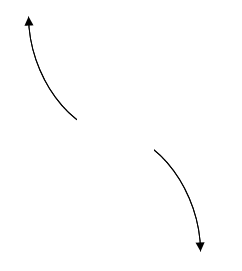
\includegraphics[width = 0.3\textwidth]{../Figures/polyEndBehaviorAC.png}\item 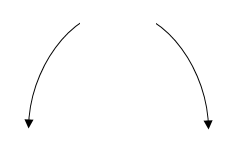
\includegraphics[width = 0.3\textwidth]{../Figures/polyEndBehaviorBC.png}\item 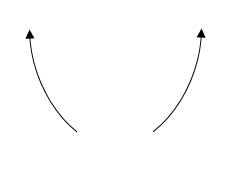
\includegraphics[width = 0.3\textwidth]{../Figures/polyEndBehaviorCC.png}\item 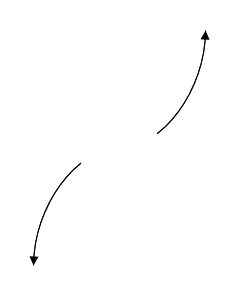
\includegraphics[width = 0.3\textwidth]{../Figures/polyEndBehaviorDC.png}\end{multicols}\item None of the above.
\end{enumerate} }
\litem{
Construct the lowest-degree polynomial given the zeros below. Then, choose the intervals that contain the coefficients of the polynomial in the form $x^3+bx^2+cx+d$.\[ -4 - 3 i \text{ and } 2 \]\begin{enumerate}[label=\Alph*.]
\item \( b \in [-7.2, -5.5], c \in [6.8, 10.2], \text{ and } d \in [48.9, 50.9] \)
\item \( b \in [-0.8, 2.4], c \in [1.5, 2.3], \text{ and } d \in [-8.1, -6.2] \)
\item \( b \in [-0.8, 2.4], c \in [-0.7, 1.3], \text{ and } d \in [-7.9, -5.2] \)
\item \( b \in [2.7, 8.3], c \in [6.8, 10.2], \text{ and } d \in [-53.6, -47.8] \)
\item \( \text{None of the above.} \)

\end{enumerate} }
\litem{
Construct the lowest-degree polynomial given the zeros below. Then, choose the intervals that contain the coefficients of the polynomial in the form $ax^3+bx^2+cx+d$.\[ \frac{7}{4}, \frac{-2}{3}, \text{ and } \frac{-4}{3} \]\begin{enumerate}[label=\Alph*.]
\item \( a \in [35, 45], b \in [129, 138], c \in [152, 162], \text{ and } d \in [53, 59] \)
\item \( a \in [35, 45], b \in [9, 14], c \in [-96, -83], \text{ and } d \in [-56, -51] \)
\item \( a \in [35, 45], b \in [83, 91], c \in [10, 14], \text{ and } d \in [-56, -51] \)
\item \( a \in [35, 45], b \in [-10, 0], c \in [-96, -83], \text{ and } d \in [53, 59] \)
\item \( a \in [35, 45], b \in [9, 14], c \in [-96, -83], \text{ and } d \in [53, 59] \)

\end{enumerate} }
\litem{
Construct the lowest-degree polynomial given the zeros below. Then, choose the intervals that contain the coefficients of the polynomial in the form $x^3+bx^2+cx+d$.\[ 3 - 3 i \text{ and } -2 \]\begin{enumerate}[label=\Alph*.]
\item \( b \in [-8, 0], c \in [5.4, 8.1], \text{ and } d \in [35, 43] \)
\item \( b \in [2, 8], c \in [5.4, 8.1], \text{ and } d \in [-39, -29] \)
\item \( b \in [1, 2], c \in [-2.7, 2.2], \text{ and } d \in [-8, -2] \)
\item \( b \in [1, 2], c \in [4.6, 5.1], \text{ and } d \in [4, 8] \)
\item \( \text{None of the above.} \)

\end{enumerate} }
\litem{
Which of the following equations \textit{could} be of the graph presented below?
\begin{center}
    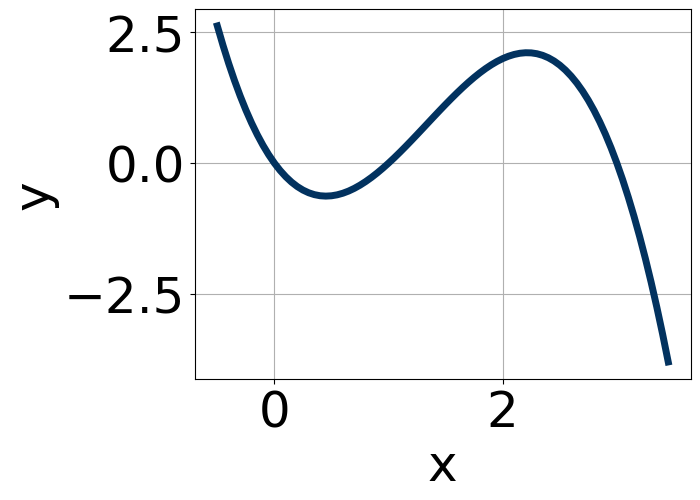
\includegraphics[width=0.5\textwidth]{../Figures/polyGraphToFunctionC.png}
\end{center}
\begin{enumerate}[label=\Alph*.]
\item \( -11x^{4} (x - 3)^{6} (x - 1)^{7} \)
\item \( -17x^{5} (x - 3)^{11} (x - 1)^{11} \)
\item \( 8x^{10} (x - 3)^{9} (x - 1)^{5} \)
\item \( 20x^{5} (x - 3)^{11} (x - 1)^{9} \)
\item \( -10x^{8} (x - 3)^{5} (x - 1)^{5} \)

\end{enumerate} }
\litem{
Describe the zero behavior of the zero $x = 8$ of the polynomial below.\[ f(x) = -8(x + 3)^{12}(x - 3)^{8}(x + 8)^{6}(x - 8)^{3} \]\begin{enumerate}[label=\Alph*.]
\begin{multicols}{2}\item 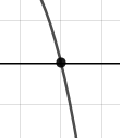
\includegraphics[width = 0.3\textwidth]{../Figures/polyZeroBehaviorCopyAC.png}\item 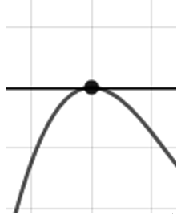
\includegraphics[width = 0.3\textwidth]{../Figures/polyZeroBehaviorCopyBC.png}\item 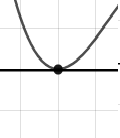
\includegraphics[width = 0.3\textwidth]{../Figures/polyZeroBehaviorCopyCC.png}\item 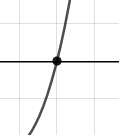
\includegraphics[width = 0.3\textwidth]{../Figures/polyZeroBehaviorCopyDC.png}\end{multicols}\item None of the above.
\end{enumerate} }
\litem{
Describe the end behavior of the polynomial below.\[ f(x) = -3(x + 3)^{2}(x - 3)^{3}(x + 2)^{5}(x - 2)^{7} \]\begin{enumerate}[label=\Alph*.]
\begin{multicols}{2}\item 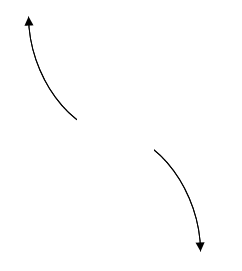
\includegraphics[width = 0.3\textwidth]{../Figures/polyEndBehaviorCopyAC.png}\item 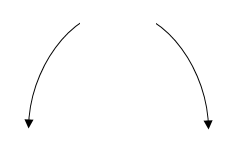
\includegraphics[width = 0.3\textwidth]{../Figures/polyEndBehaviorCopyBC.png}\item 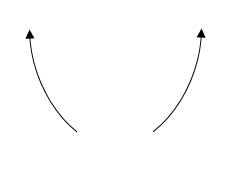
\includegraphics[width = 0.3\textwidth]{../Figures/polyEndBehaviorCopyCC.png}\item 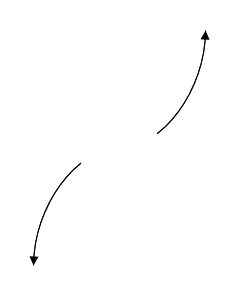
\includegraphics[width = 0.3\textwidth]{../Figures/polyEndBehaviorCopyDC.png}\end{multicols}\item None of the above.
\end{enumerate} }
\litem{
Which of the following equations \textit{could} be of the graph presented below?
\begin{center}
    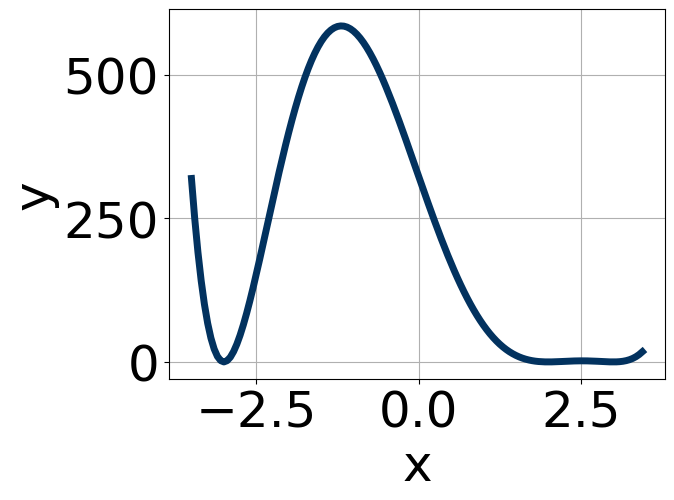
\includegraphics[width=0.5\textwidth]{../Figures/polyGraphToFunctionCopyC.png}
\end{center}
\begin{enumerate}[label=\Alph*.]
\item \( 17(x + 3)^{10} (x - 3)^{6} (x - 2)^{8} \)
\item \( -18(x + 3)^{10} (x - 3)^{10} (x - 2)^{11} \)
\item \( -18(x + 3)^{10} (x - 3)^{4} (x - 2)^{4} \)
\item \( 10(x + 3)^{4} (x - 3)^{7} (x - 2)^{5} \)
\item \( 4(x + 3)^{4} (x - 3)^{4} (x - 2)^{5} \)

\end{enumerate} }
\litem{
Describe the zero behavior of the zero $x = 4$ of the polynomial below.\[ f(x) = 4(x + 9)^{4}(x - 9)^{2}(x + 4)^{13}(x - 4)^{8} \]\begin{enumerate}[label=\Alph*.]
\begin{multicols}{2}\item 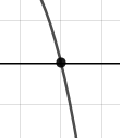
\includegraphics[width = 0.3\textwidth]{../Figures/polyZeroBehaviorAC.png}\item 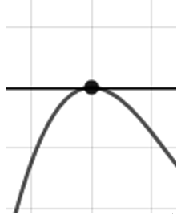
\includegraphics[width = 0.3\textwidth]{../Figures/polyZeroBehaviorBC.png}\item 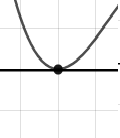
\includegraphics[width = 0.3\textwidth]{../Figures/polyZeroBehaviorCC.png}\item 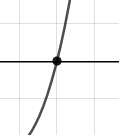
\includegraphics[width = 0.3\textwidth]{../Figures/polyZeroBehaviorDC.png}\end{multicols}\item None of the above.
\end{enumerate} }
\end{enumerate}

\end{document}